%%%%%%%%%%%%%%%%%%%%%%%%%%%%%%%%%%%%%%%%%%%%%%%%%%%%%%%%%%%%%%%%%%%%%%%%%%%%%%%%
% Note : Cette activité n'est pas de moi, et a été copiée de manière éhontée
% à ma tutrice de stage.
%%%%%%%%%%%%%%%%%%%%%%%%%%%%%%%%%%%%%%%%%%%%%%%%%%%%%%%%%%%%%%%%%%%%%%%%%%%%%%%%
\documentclass[12pt, aspectratio=43]{beamer}

\usepackage{pablo-beamer}

\newcommand{\drapeau}[1]{
  \draw (0,0) -- ++(0,2) -- ++(1,0) -- ++(0, -1) -- ++(-1, 0);
  \draw (0,0) node[right]{(#1)};
}

\institute{Lycée Marie Curie}
\date{2015}
\logo{}
\title{Un nouveau déplacement}

\begin{document}


\section{Exercice 1}
\begin{frame}
  \begin{center}
    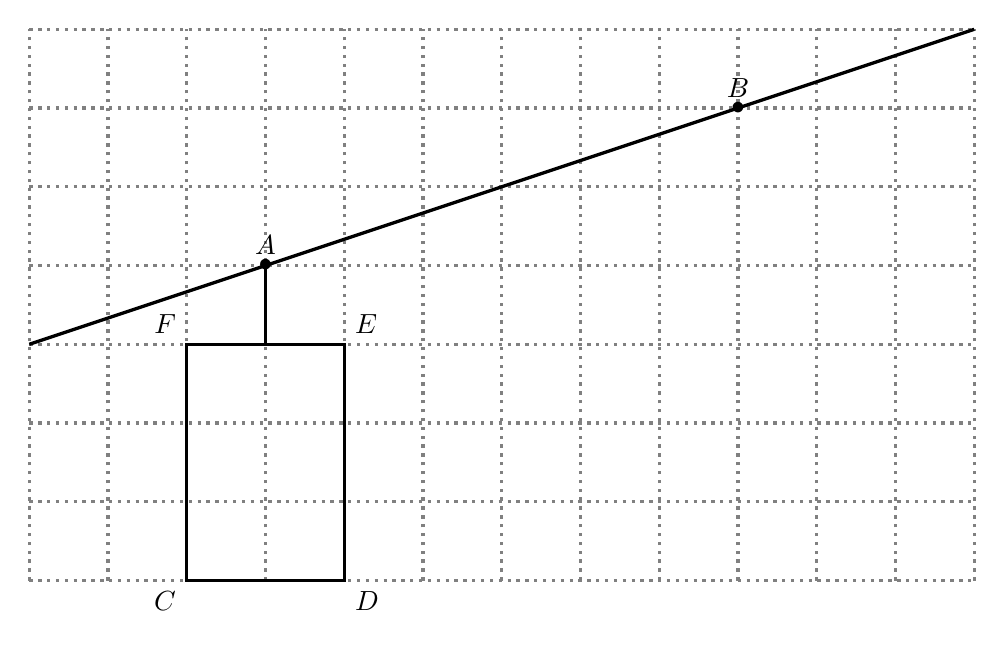
\begin{tikzpicture}[very thick,scale=1]
      \draw[dotted, gray] (0,0) grid (12, 7);
      \draw (2, 0)  node[below left]{$C$}
      -- ++(2, 0)  node[below right]{$D$}
      -- ++(0, 3)  node[above right]{$E$}
      -- ++(-2, 0) node[above left]{$F$}
      -- cycle;
      \draw (3,3) -- (3,4);
      \draw (0,3) -- (12, 7);

      \draw (3,4) node{$\bullet$} node[above]{$A$};
      \draw (9,6) node{$\bullet$} node[above]{$B$};
    \end{tikzpicture}
  \end{center}
\end{frame}

\section{Exercice 2}
\begin{frame}
  \begin{tabular}{c|c|c}
    a)
    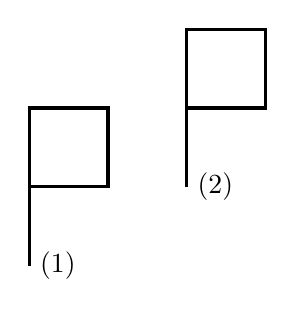
\begin{tikzpicture}[very thick]
      \drapeau{1}
      \begin{scope}[shift={(2,1)}]
        \drapeau{2}
      \end{scope}
    \end{tikzpicture}
    &
    b)
    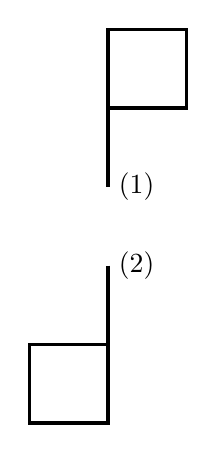
\begin{tikzpicture}[very thick]
      \drapeau{1}
      \begin{scope}[shift={(0,-1)},rotate=180]
        \drapeau{2}
      \end{scope}
    \end{tikzpicture}
    &
    c)
    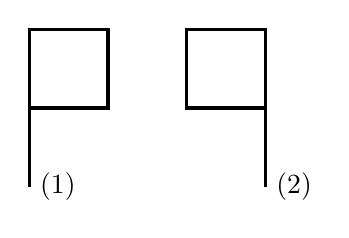
\begin{tikzpicture}[very thick]
      \drapeau{1}
      \begin{scope}[xscale=-1,shift={(-3,0)}]
        \drapeau{2}
      \end{scope}
    \end{tikzpicture}
    \\
    \hline

    d)
    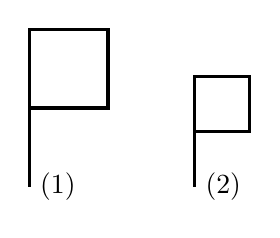
\begin{tikzpicture}[very thick]
      \drapeau{1}
      \begin{scope}[scale=.7,shift={(3,0)}]
        \drapeau{2}
      \end{scope}
    \end{tikzpicture}
    &
    e)
    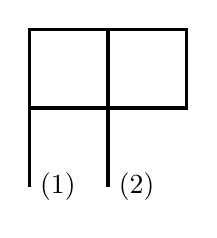
\begin{tikzpicture}[very thick]
      \drapeau{1}
      \begin{scope}[shift={(1,0)}]
        \drapeau{2}
      \end{scope}
    \end{tikzpicture}
    &
    f)
    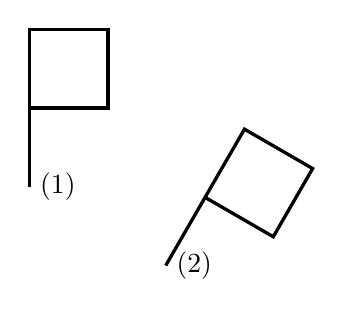
\begin{tikzpicture}[very thick]
      \drapeau{1}
      \begin{scope}[rotate=-30,shift={(2,0)}]
        \drapeau{2}
      \end{scope}
    \end{tikzpicture}

  \end{tabular}
\end{frame}

\section{Exercice 3}
\begin{frame}
  \begin{center}
    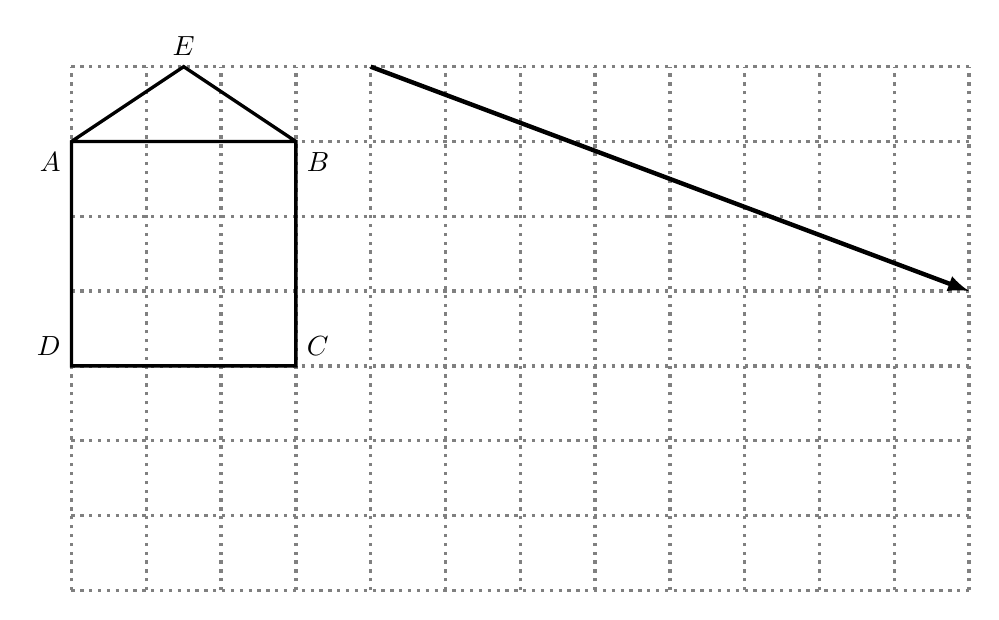
\begin{tikzpicture}[very thick, scale=.95]
      \draw[dotted, gray] (0,0) grid (12, 7);
      \draw (0, 6)  node[below left]{$A$}
      -- ++(3, 0)  node[below right]{$B$}
      -- ++(0, -3)  node[above right]{$C$}
      -- ++(-3, 0) node[above left]{$D$}
      -- ++(0, 3)
      -- ++(1.5, 1) node[above]{$E$}
      -- ++(1.5, -1);

      \draw[-latex, ultra thick] (4, 7) -- (12, 4);
    \end{tikzpicture}
  \end{center}
\end{frame}
\end{document}
